% (c) 2012 Silvia Cibola - silvia.cibola@gmail.com
% (c) 2012 - 2014 Dimitrios Vrettos - d.vrettos@gmail.com

\section{Esercizi}

\subsection{Esercizi dei singoli capitoli}

\subsubsection*{\thechapter.1 - Prime definizioni}
\begin{esercizio}
\label{ese:F.1}
Segnate nel piano dotato di riferimento cartesiano ortogonale i vettori~$\vec{v}(1;2)$ e~$\vec{w}(3;-1)$. Possiamo affermare che~$|\vec{w}|=2 \cdot |\vec{v}|$?
\end{esercizio}

\subsubsection*{\thechapter.2 - Operazioni con i vettori}
\begin{esercizio}
\label{ese:F.2}
Provate a giustificare la seguente affermazione: l'operazione di addizione definita secondo la regola del parallelogramma gode della proprietà commutativa.
\end{esercizio}

\begin{esercizio}
\label{ese:F.3}
Determinate il vettore~$\vec{z}=\vec{u}+\vec{w}$ essendo~$\vec{u}(-1;-3)$ e~$\vec{v}(2;-1)$. Determinate inoltre il modulo di~$\vec{z}$ e la sua direzione.
Potete affermare che~$|\vec{z}|=|\vec{u}|+|\vec{w}|$?
\end{esercizio}

\begin{esercizio}
\label{ese:F.4}
Nel riferimento cartesiano ortogonale riportato di seguito sono rappresentati i vettori~$\vec{u}$ e~$\vec{v}$. Completate:

\begin{enumeratea}
\item il vettore~$\vec{u}$ è applicato all'origine e ha componenti~$\ldots$;
\item il vettore~$\vec{v}$ ha il primo estremo in~$B(\ldots;\ldots)$ e il secondo in~$\ldots$, pertanto le sue componenti sono~$\ldots$;
\item $m_{\vec{u}}=\ldots$ e~$m_{\vec{v}}=\ldots$, pertanto essi sono~$\ldots$;
\item $|\vec{u}|=\ldots$ e~$|\vec{v}|=\ldots$;
\item determinare~$r$ in modo che~$\vec{v}=r \cdot \vec{u}$.
\end{enumeratea}
\begin{center}
 % (c) 2012 Dimitrios Vrettos - d.vrettos@gmail.com

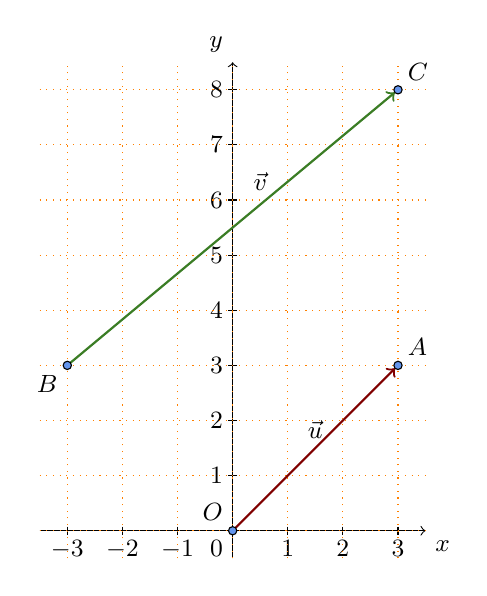
\begin{tikzpicture}[x=7mm,y=7mm, font=\small]

  \begin{scope}[->]
    \draw (-3.5,0) -- (3.5,0) node [below right] {$x$};
    \draw (0,-.5) -- (0,8.5) node[above left] {$y$};
  \end{scope}

  \foreach \x/\xtext in {-3/-3,-2/-2,-1/-1,1/1,2/2,3/3}{
    \node[below] at (\x,0) {$\xtext$};
    \draw (\x,1.5pt) -- (\x,-1.5pt);}
  \foreach \y/\ytext in {1/1,2/2,3/3,4/4,5/5,6/6,7/7,8/8}{
    \node[left] at (0,\y) {$\ytext$};
    \draw (1.5pt,\y) -- (-1.5pt,\y);}
  \node[below left] at (0,0) {$0$};

  \begin{scope}[dotted, orange, step=7mm]
    \draw (-3.5,-.5) grid (3.5,8.5);
  \end{scope}

  \begin{scope}[thick, ->,shorten >=1.5pt]
	\draw[Maroon] (0,0) -- (3,3);  
	\draw[OliveGreen](-3,3) -- (3,8);
      \end{scope}
 

\begin{scope}[fill=CornflowerBlue, draw=black]
\filldraw (0,0) circle (1.5pt)node [above left]{$O$};
\filldraw (3,3) circle (1.5pt)node [above right]{$A$};
\filldraw (-3,3) circle (1.5pt)node [below left]{$B$};
\filldraw (3,8) circle (1.5pt) node [above right]{$C$};
\end{scope}
\node[above] at (1.5,1.5) {$\vec{u}$};
\node[above] at (.5,6) {$\vec{v}$};
\end{tikzpicture}
\end{center}

\end{esercizio}

\begin{esercizio}
\label{ese:F.5}
Determinate le componenti del vettore~$\vec{w}=2 \cdot \vec{v}$ essendo~$\vec{v}(\frac{3}{2};-2)$. Verificate che~$\vec{w}$ e~$\vec{v}$ hanno stessa direzione
e~$|\vec{w}|=2 \cdot |\vec{v}|$.
\end{esercizio}

\begin{esercizio}
\label{ese:F.6}
Verificate che~$\frac{3}{2} \cdot (\vec{x}+\vec{y})=\frac{3}{2}\vec{x}+\frac{3}{2}\vec{y}$ essendo~$\vec{x}(-\frac{5}{4};1)$ e~$\vec{y}(4;-1)$.
\end{esercizio}
\pagebreak
\subsubsection*{\thechapter.3 - Dipendenza e indipendenza lineare}
\begin{esercizio}
\label{ese:F.7}
Completate le scritture:
\begin{multicols}{2}
\begin{enumeratea}
\item $\vec{v}(-\sqrt{2};\frac {5}{4})=\ldots \cdot \vec{i}+\ldots \cdot \vec{j}$;
\item $\vec{u}(1;-1)=\ldots \cdot \vec{i}+\ldots \cdot \vec{j}$;
\item $\vec{h}(\ldots;\ldots)=\frac {\sqrt{3}}{3} \cdot \vec{i}-9 \cdot \vec{j}$;
\item $\vec{z}(\ldots;\ldots)=\frac {3 \sqrt{5}}{3} \cdot \vec{i}$;
\end{enumeratea}
\end{multicols}
\end{esercizio}

\begin{esercizio}
\label{ese:F.8}
\begin{multicols}{2}
 Dati i vettori della figura a fianco, applicate il metodo geometrico per determinare i vettori che permettono di scrivere~$\vec{w}$ come combinazione lineare degli altri due.
Riprendete questi stessi vettori e determinate i vettori che permettono di scrivere~$\vec{v}$ come combinazione lineare degli altri due. In maniera analoga, determinate i vettori che permettono di scrivere~$\vec{u}$ come combinazione lineare degli altri due ($\vec{v}$ e $\vec{w}$).
\begin{center}
% (c) 2012 Dimitrios Vrettos - d.vrettos@gmail.com

\begin{tikzpicture}[x=10mm,y=10mm, font=\small, every state/.style={draw=CornflowerBlue, minimum size=0pt}, every loop/.style={draw=Maroon}]
\draw (0,0) circle (1.5);
\node at (1.3,1.5) {$A$};
\node at (0,-2) {caso 1};
\node[state] (1) at (-1,0) {$a$};
\node[state] (2) at (.5,.7) {$b$};
\node[state] (3) at (1,0) {$c$};
\node[state] (4) at (-.6,-.7) {$d$};
\node[state] (5) at (.5,-.5) {$e$};
\node[state] (6) at (-.2,.2) {$f$};
\node[state] (7) at (.2,-1.1) {$g$};
\node[state] (8) at (-.4,1.1) {$h$};
\begin{scope}[->]
\path (1) edge[loop above] node{} ()
	(2) edge[loop above] node{} ()
   (6) edge[loop below] node {} ()
(3) edge[loop above] node{} ()
(4) edge[loop left] node{} ()
(7) edge[loop right] node{} ();

\end{scope}
\begin{scope}[-, Maroon]
\draw (1)--(8);
\draw (1)--(6);
\draw (8)--(6);

\draw (2)--(3);
\draw (2)--(5);
\draw (3)--(5);

\draw (4)--(7);
\end{scope}

 \begin{scope}[xshift=32mm]
\draw (0,0) circle (1.5);
\node at (1.3,1.5) {$B$};
\node at (0,-2) {caso 2};
\node[state] (1) at (-1,0) {$a$};
\node[state] (2) at (.5,.7) {$b$};
\node[state] (3) at (1,0) {$c$};
\node[state] (4) at (-.6,-.7) {$d$};
\node[state] (5) at (.5,-.5) {$e$};
\node[state] (6) at (-.2,.2) {$f$};
\node[state] (7) at (.2,-1.1) {$g$};
\node[state] (8) at (-.4,1.1) {$h$};
\begin{scope}[->]
\path (1) edge[loop above] node{} ()
	(2) edge[loop above] node{} ()
   (6) edge[loop below] node {} ()
(3) edge[loop above] node{} ()
(4) edge[loop left] node{} ()
(7) edge[loop right] node{} ()
(5) edge[loop right] node{} ()
(8) edge[loop right] node{} ();

\end{scope}
\begin{scope}[-, Maroon]
\draw (1)--(8);
\draw (1)--(6);
\draw (8)--(6);

\draw (2)--(3);
\draw (2)--(5);
\draw (3)--(5);

\draw (4)--(7);
\end{scope}
 \end{scope}

 \begin{scope}[xshift=64mm]
\draw (0,0) circle (1.5);
\node at (1.3,1.5) {$C$};
\node at (0,-2) {caso 3};
\node[state] (1) at (-1,0) {$a$};
\node[state] (2) at (.5,.7) {$b$};
\node[state] (3) at (1,0) {$c$};
\node[state] (4) at (-.6,-.7) {$d$};
\node[state] (5) at (.5,-.5) {$e$};

\begin{scope}[->]
\path (1) edge[loop above] node{} ()
	(2) edge[loop above] node{} ()
(3) edge[loop above] node{} ()
(4) edge[loop left] node{} ()
(5) edge[loop right] node{} ();

\end{scope}
\begin{scope}[-, Maroon]
\draw (1)--(2);
\draw (2)--(3);
\draw (4)--(5);
\end{scope}
 \end{scope}

 \begin{scope}[xshift=96mm]
\draw (0,0) circle (1.5);
\node at (1.3,1.5) {$D$};
\node at (0,-2) {caso 4};
\node[state] (1) at (-1,0) {$a$};
\node[state] (2) at (.5,.7) {$b$};
\node[state] (3) at (1,0) {$c$};
\node[state] (4) at (-.6,-.7) {$d$};
\node[state] (6) at (.5,-.5) {$f$};
\begin{scope}[->]
\path (1) edge[loop above] node{} ()
	(2) edge[loop above] node{} ()
   (6) edge[loop below] node {} ()
(3) edge[loop above] node{} ()
(4) edge[loop left] node{} ();

\end{scope}
\begin{scope}[->, Maroon]
\draw (3)--(1);
\draw (2)--(1);
\draw (2)--(3);
\end{scope}
 \end{scope}
\end{tikzpicture}
\end{center}
\end{multicols}
\end{esercizio}

\begin{esercizio}
\label{ese:F.9}
I vettori dell'esercizio precedente sono linearmente dipendenti?
\end{esercizio}

\begin{esercizio}
\label{ese:F.10}
Spiegate perché i tre vettori~$\vec{v}(1;2)$, $\vec{u}(3;1)$ e~$\vec{w}(-3;-6)$ sono linearmente dipendenti.
\end{esercizio}

